\documentclass[../main.tex]{subfiles}
\graphicspath{{\subfix{../images/}}} % Images path

\begin{document}

\section{Visual Vocabulary Construction}\label{sec:visual-vocabulary-construction}

The process of building a visual vocabulary can be split in two main steps: 

\begin{enumerate}
  \item \textbf{Feature extraction}: sampling of SIFT descriptors from train images.
  \item \textbf{Clustering}: grouping of the extracted descriptors into $k$ clusters.
\end{enumerate}

\subsection{Feature Extraction}\label{subsec:feature-extraction}

The first step in building a visual vocabulary is to extract features from the images in the training set. 
In this case, SIFT descriptors are used as features and they have been extracted following two different approaches:

\begin{enumerate}
  \item using the \bft{SIFT detector}: the SIFT detector is used to detect keypoints in the images and then the corresponding SIFT descriptors are computed on these keypoints.
  \item sampling on a \bft{dense regular grid}: following the approach adopted by \itt{Lazebnik et al.} [TOOD: add reference], SIFT descriptors can also be computed from keypoints sampled on a regular dense grid over each image. Following the approach of the paper, a regular grid with spacing of $8$ pixels between each keypoint has been used.
\end{enumerate}

As highlighted by \itt{Lazebnik et al.} [TOOD: add reference] reporting the original evaluation from \itt{Fei-Fei and Perona} [TOOD: add reference], sampling descriptors from a regular grid should intuitively work better from scene classification tasks, as this method allows to capture uniform regions such as sky, calm water, or road surfaces.\\
Both sampling methods have been tested and compared, with the results shown in later section~\ref{sec:results}. For the first approach, the SIFT detector has been initialized to retain only the best $500$ features in each image resulting in a total of $\num{593006}$ keypoints, while for the second approach $\num{1482434}$ keypoints have been collected.\\
Notice that with both approaches the exact number of keypoints extracted in each image can change from one image to another. In the first case, this is due to the content of the images and the actual features present in them\footnote{Intuitively, images with a lot of texture or with a lot of edges will have more keypoints than images with uniform regions such as sky or water.}, while in the second case this is due to the different sizes and aspect ratios of the images in the dataset. Figure~\ref{fig:keypoints-example} shows an example of this phenomenon, where a different number of keypoints has been detected by the SIFT detector in two different images.

\begin{figure}[H]
  \centering
  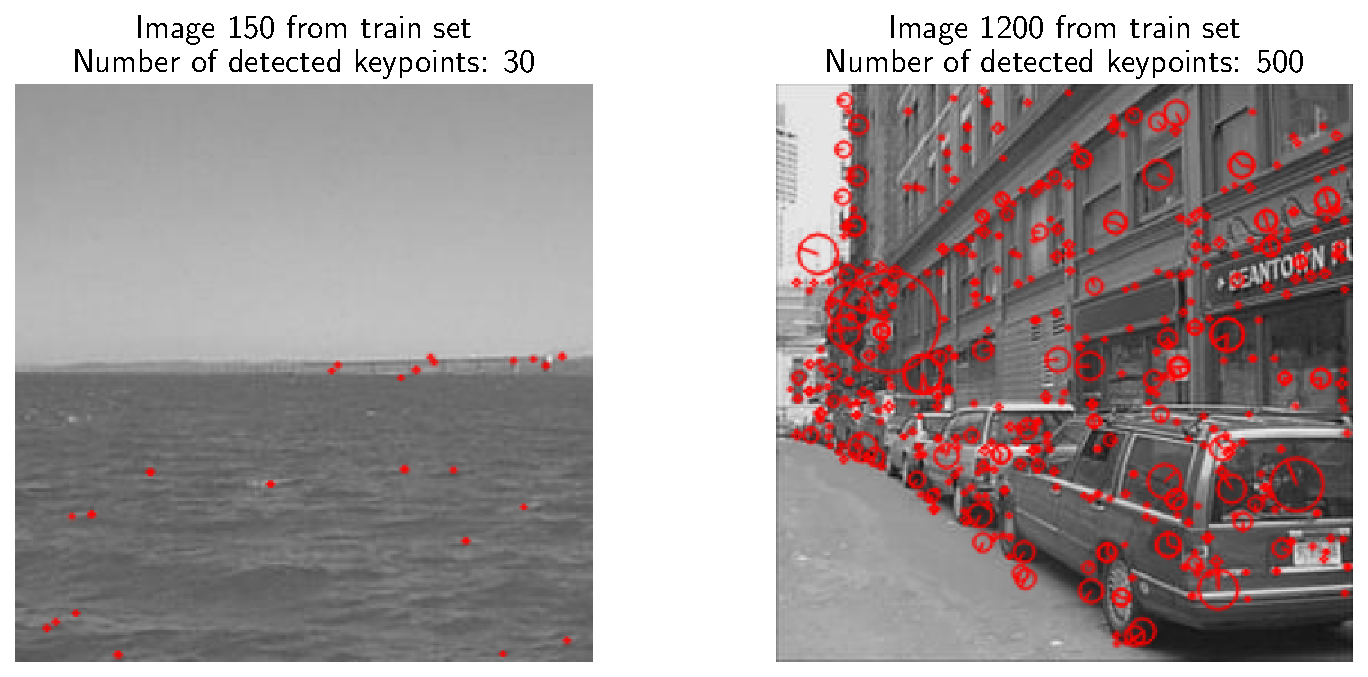
\includegraphics[width=\textwidth]{keypoints.pdf}
  \caption{Example of keypoints detected by the SIFT detector in two different images. In the left side image only $30$ keypoints have been detected, while in the right side image all the desired $500$ keypoints have been detected.}
  \label{fig:keypoints-example}
\end{figure}


\subsection{Clustering}\label{subsec:clustering}

Following the previous step, clustering has been performed on a random subset of extracted SIFT descriptors to build the visual vocabulary. The size of the subset has been fixed to $\num{10000}$ for descriptors sampled using SIFT detector and to $\num{25000}$ for descriptors sampled on a regular grid. This has been done to approximatively maintain the same ratio between the total number of sampled descriptors and the number of descriptors used for clustering in the two cases.\\
In paticular, the \itt{k-means} algorithm has been used to cluster the descriptors into $K$ clusters, where $K$ is the size of the visual vocabulary.\\
For this purpose, different values of $K$ have been tested, ranging from $K=50$ to $K=1000$. After some tests, the value of $K=400$ has been fixed to build the visual vocabulary. This choice is motivated by two main reasons. First, since the value of the silhouette score decreases noticeably after $K=400$ as it's possible to see in figure~\ref{fig:silhouette-score}, this value has been chosen as a good trade-off between the quality of the clustering and the computational cost of the clustering process. Second, considering the purpose of this project, the value of $K=400$ allows for a direct comparison with the results reported in the original paper by \itt{Lazebnik et al.} [TOOD: add reference], where the same value has been used.\\
After the clustering process, the obtained centroids representation the visual words of the vocabulary will be $128$-dimensional vectors.

% \begin{figure}[H]
%   \centering
%   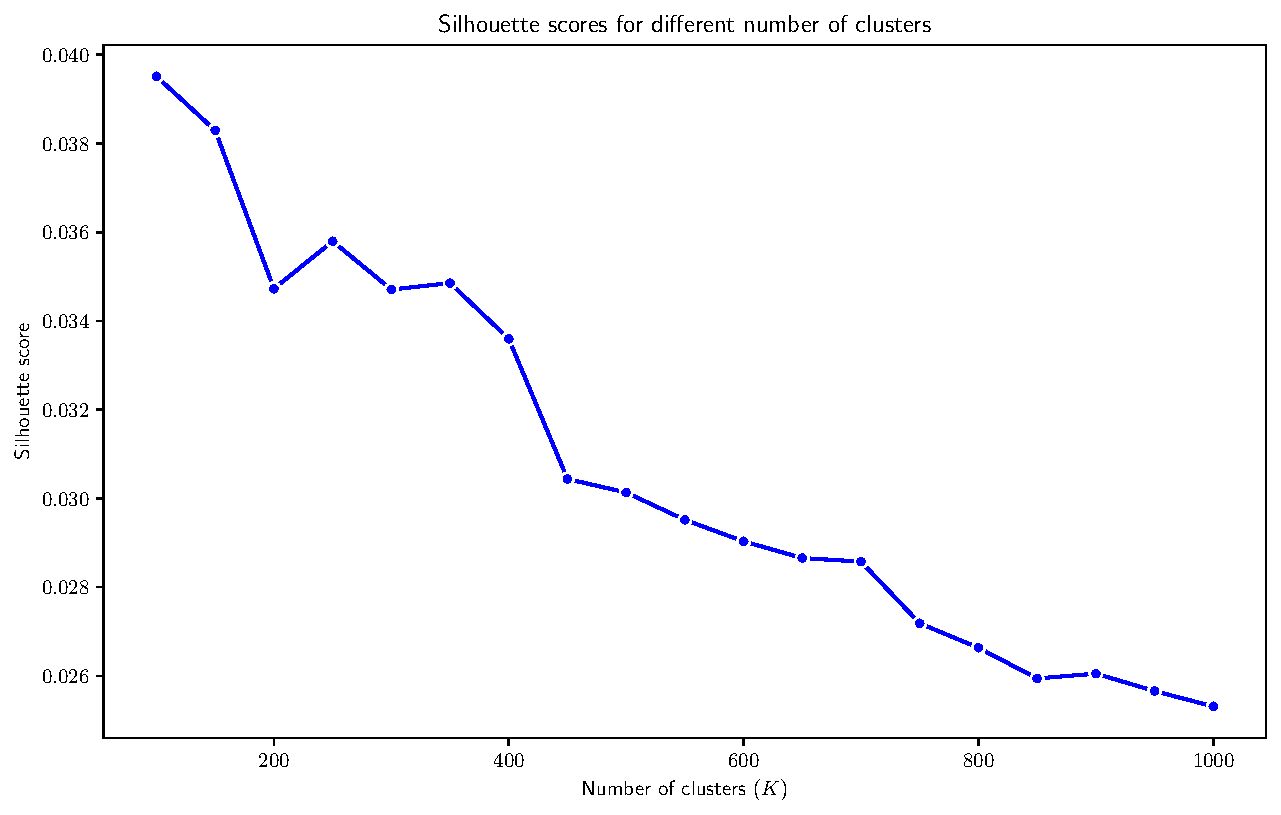
\includegraphics[width=\textwidth]{silhouette_scores.pdf}
%   \caption{Silhouette score for different values of $K$. As expected the value decreases with the increase of $K$. A relatively significant decrease is observed after $K=400$.}
%   \label{fig:silhouette-score}
% \end{figure}

\begin{figure}[H]
  \centering
  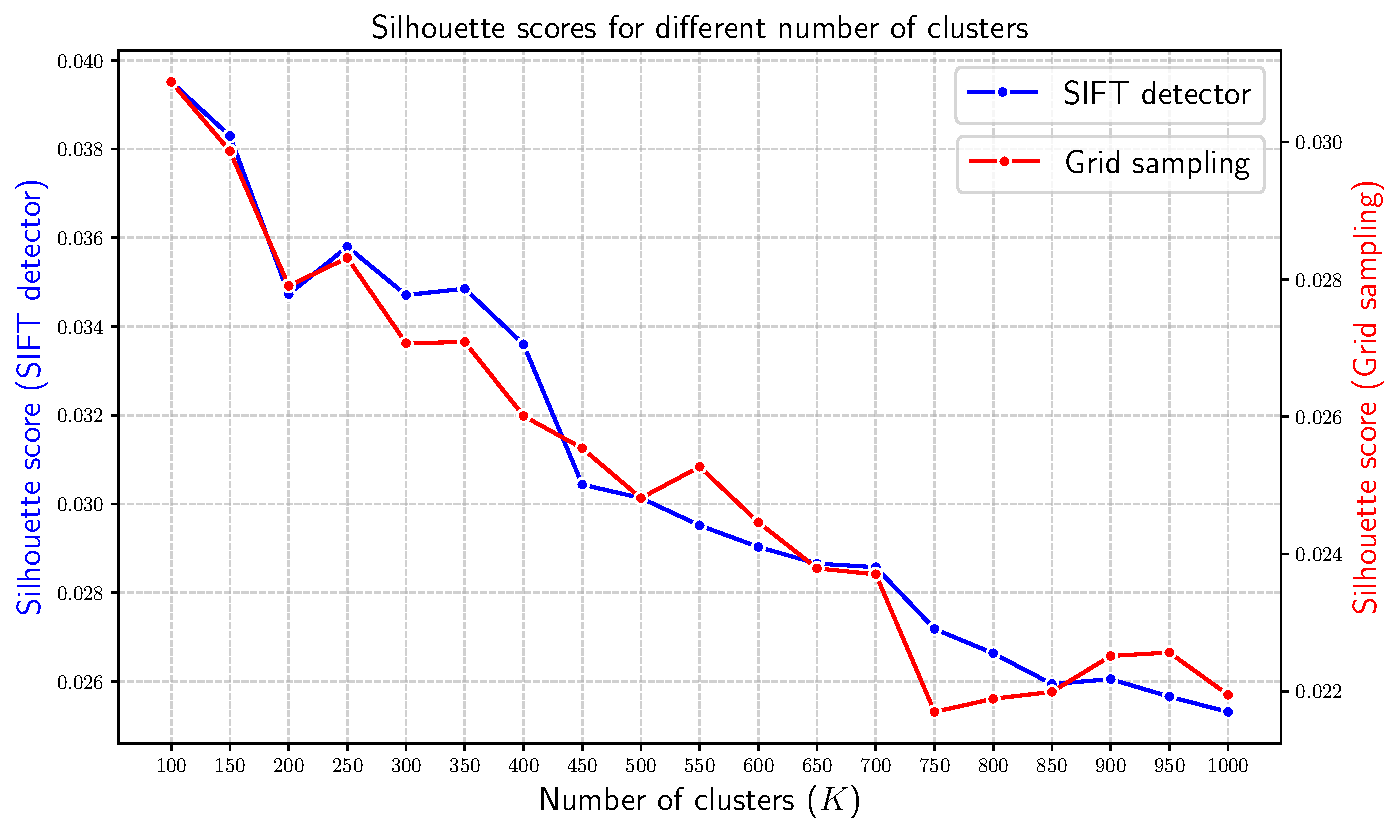
\includegraphics[width=\textwidth]{silhouette_scores_comparison.pdf}
  \caption{Silhouette score for different values of $K$ resulting from clustering on SIFT descriptors sampled using the SIFT detector (blue) and on a regular grid (red).As expected the value decreases with the increase of $K$. Relatively significant decreases are observed after $K=200$ and $K=400$ for the two cases.}
  \label{fig:silhouette-score}
\end{figure}

\end{document}

